

\section{Experiments}
\label{experiments}
For our experiments, our training data is given by $(x_i, f(x_i))$, where $x_i$ are randomly chosen from a standard Gaussian in $\R^d$ and $f$ is a randomly generated neural network with weights chosen from a standard Gaussian. We run gradient descent (Algorithm \ref{GD}) on the empirical loss, with stepsize around $\alpha = 10^{-5}$, for $T = 10^6$ iterations. The nonlinearity used at each node is sigmoid, and further, unlike the assumptions in the theoretical analysis, the top node is a sign function outputing binary variable. Thus a random guess for the network will result in a error rate of $0.5$ ($50\%$) Our experiments show that for depth-2 neural networks, even with non-linear outputs, the training error starting from a value of about $50\%$ diminishes quickly to under $2\%$. This seems to hold even when the width, the number of hidden nodes, is substantially increased (even up to 125 nodes), but depth is held constant; although as the number of nodes increases, the rate of decrease is slower. This substantiates our claim that depth-2 neural networks are learnable.

However, it seems that for depth greater than 2, the test error becomes significant  when width is high. When the width is a small constant, the increase in depth also impedes the learnability of the neural network and the training error does not get close enough to 0. It seems that for neural networks with greater depth, positive convergence results in practice are elusive.
\begin{table}[tb]
\caption{Test Error of Learning Neural Networks of Various Depth and Width}
\vskip 0.1in
\begin{center}
\begin{small}
\begin{sc}
\begin{tabular}{
  p{\dimexpr.2\linewidth-2\tabcolsep-1.3333\arrayrulewidth}|% column 0
   |p{\dimexpr.2\linewidth-2\tabcolsep-1.3333\arrayrulewidth}% column 1
  |p{\dimexpr.2\linewidth-2\tabcolsep-1.3333\arrayrulewidth}% column 2
  |p{\dimexpr.2\linewidth-2\tabcolsep-1.3333\arrayrulewidth}% column 3
  |p{\dimexpr.2\linewidth-2\tabcolsep-1.3333\arrayrulewidth}% column 4
   |p{\dimexpr.2\linewidth-2\tabcolsep-1.3333\arrayrulewidth}% column 5
  }
   \hline 
           & Width 5   &  Width 10   & Width 20 & Width 40     \\ \hline 
    Depth 2 & 0.0015   & 0.0017      &   0.0018 & 0.0019 \\ \hline
    Depth 3 & 0.0033   & 0.0264        &   0.1503 & 0.2362 \\ \hline
    Depth 5 & 0.0036   & 0.0579        &   0.2400 & 0.4397 \\ \hline
    Depth 9 & 0.0085   & 0.1662        &   0.4171 & 0.6071 \\ \hline
    Depth 17 & 0.0845   & 0.3862        &   0.4934 & 0.5777 \\ \hline
\end{tabular}
\end{sc}
\end{small}
\end{center}
\vskip -0.1in
\end{table}


% \begin{figure}[tb]
% \begin{center}


\begin{figure}[h]
\vskip 0.1in
  \centering
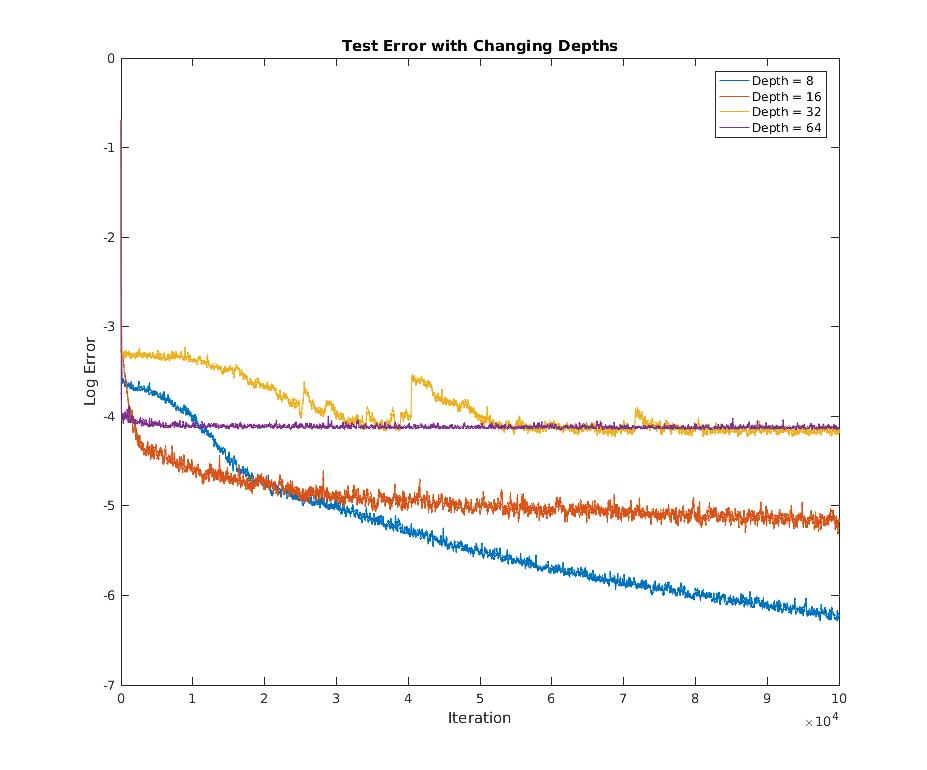
\includegraphics[width = 2.5in]{plotChangeDepth.jpg}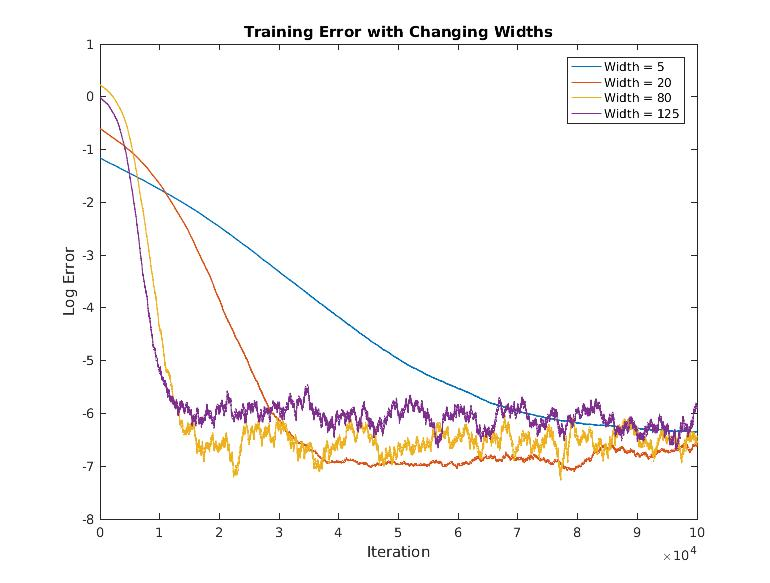
\includegraphics[width = 2.71in]{plotChangeWidth.jpg}
\caption{Left:Test Error of Networks of Varying Depth. Right: Test Error of Networks of Varying Width.}
%  \fbox{\rule[-.5cm]{0cm}{4cm} \rule[-.5cm]{4cm}{0cm}}
\end{figure}
\Snote{Do we need the figure? Figures should be the same size. Make the fonts larger, they
  are hard to read. The figure caption should read training error
  rather than test error.}
% \end{center}
\vskip -0.1in
We note that we have been using training error as a measure of
success, but it's possible that the true underlying parameters are not
learned. If our loss function were strongly convex, small training
error would imply a small norm in the parameter space. 



%%% Local Variables:
%%% mode: latex
%%% TeX-master: "icmlpaper2017.tex"
%%% End: